% Compte rendu Courpain (L3, 2021). Compiler dans outils/rapports/courpain :
%   Rscript figures.R && ../compiler.sh courpain
\documentclass[11pt,a4paper]{article}
\usepackage{../rapport-portfolio}
\definecolor{themehex}{HTML}{3F7A3A}\colorlet{theme}{themehex}
\addbibresource{references.bib}

\titrerapport{Diversité floristique et habitats de l'ancienne carrière de Courpain (Loiret)}
\titrecourt{Habitats de la carrière de Courpain}
\soustitre{Relevés phytosociologiques, cartographie des habitats et analyses multivariées}
\auteurs{Jérémy Genty et Vélinka Beaubois}
\cadre{Licence 3 BO3 · UE Phytosociologie et géomatique · Université d'Orléans}
\annee{Compte rendu de travaux pratiques · 2021}
\motcle{Phytosociologie et géomatique}
\visuel{\photogarde{figures/photo_aerienne.jpg}}
\creditvisuel{Le plan d'eau de Courpain vu du ciel (photo : Luc-André Pineau, juin 2016).}

\begin{document}
\pagedegarde

\enbref{Sur 17~ha réaménagés, le plan d'eau (5,1~ha) et les pelouses et prairies (4,2~ha) dominent. Les 45 relevés de 2018 à 2021 se répartissent en trois groupes, ordonnés par le gradient d'humidité : grèves humides à annuelles (thérophytes), mégaphorbiaie à hautes herbes et jeunes saules et peupliers, pelouses sèches sableuses et acides dominées par les vivaces (hémicryptophytes).}

\section{Introduction}
L'observatoire de Courpain est une ancienne carrière d'extraction de granulats de 17~ha, fermée en 2007 puis réaménagée par l'Institut d'écologie appliquée. Le réaménagement visait l'appropriation du site par la faune et la flore locales et la création d'un observatoire écologique et ornithologique. Depuis 2015, la gestion est confiée à la Maison de Loire du Loiret, associée au Conseil départemental depuis 2016, autour de trois axes : préserver les oiseaux et leurs habitats, améliorer les connaissances écologiques du site, et l'ouvrir au public.

Ce travail caractérise le site sur le plan du milieu physique et de la flore. Les relevés, faits le long de transects en milieu sec, humide et en mégaphorbiaie, sont compilés en un tableau brut. Ce tableau est analysé par analyse factorielle des correspondances (AFC), classification ascendante hiérarchique (CAH), histogrammes de fréquence et spectres biologiques, et les habitats sont cartographiés sous QGIS.

\section{Description du site}
\subsection{Milieu physique}
Nous avons d'abord décrit le relief et l'exposition de la station, positionné celle-ci à la boussole par triangulation, puis levé sa topographie à la règle graduée et à l'altimètre. Des carottes de sol prélevées à plusieurs profondeurs, disposées dans une gouttière, ont permis de déterminer la couleur (charte Munsell), la texture (test au toucher) et le pH (papier indicateur, figure~\ref{fig:sol}) :
\begin{itemize}
\item horizon 1 (0 à 20~cm) : limon sableux, couleur 10YR 3/3, pH 5 ;
\item horizon 2 (20 à 70~cm) : sable et cailloux, couleur 5YR 4/5, pH 5.
\end{itemize}
Le sol est donc sableux, filtrant et acide.

\begin{figure}[ht]
\centering
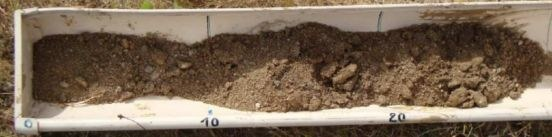
\includegraphics[height=24mm]{figures/sol_gouttiere.jpg}\hspace{2mm}%
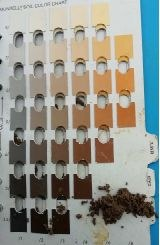
\includegraphics[height=24mm]{figures/sol_munsell.jpg}\hspace{2mm}%
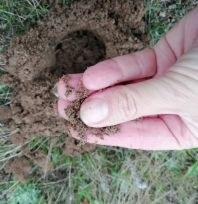
\includegraphics[height=24mm]{figures/sol_texture.jpg}\hspace{2mm}%
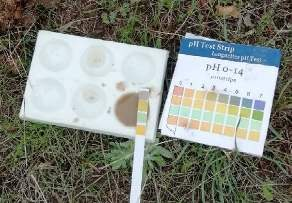
\includegraphics[height=24mm]{figures/sol_ph.jpg}
\caption{Analyse du sol : carotte disposée en gouttière, charte Munsell, test de texture et mesure du pH.}
\label{fig:sol}
\end{figure}

\noterevision{Note de révision (2026) : la version de 2021 indiquait des profondeurs en mètres (0 à 20~m) et des codes Munsell mal transcrits (« 104R », « 54R ») ; ils sont corrigés ici en centimètres et en notation Munsell standard, d'après la lecture la plus probable.}

\subsection{Carte des habitats}
Les points GPS des relevés de 2018 à 2021 ont été reportés sous QGIS, avec les contours des habitats (figure~\ref{fig:carte}). Chaque relevé est codé par l'année, le transect et la position (par exemple 21T1a : 2021, transect~1, point~a). Le plan d'eau occupe la plus grande surface (5,1~ha), suivi des pelouses et prairies (4,2~ha). Autour de l'eau, la végétation change avec la distance à la berge : grèves, roselière, ripisylve, puis lande à genêts et pelouses (tableau~\ref{tab:surfaces}).

\begin{figure}[ht]
\centering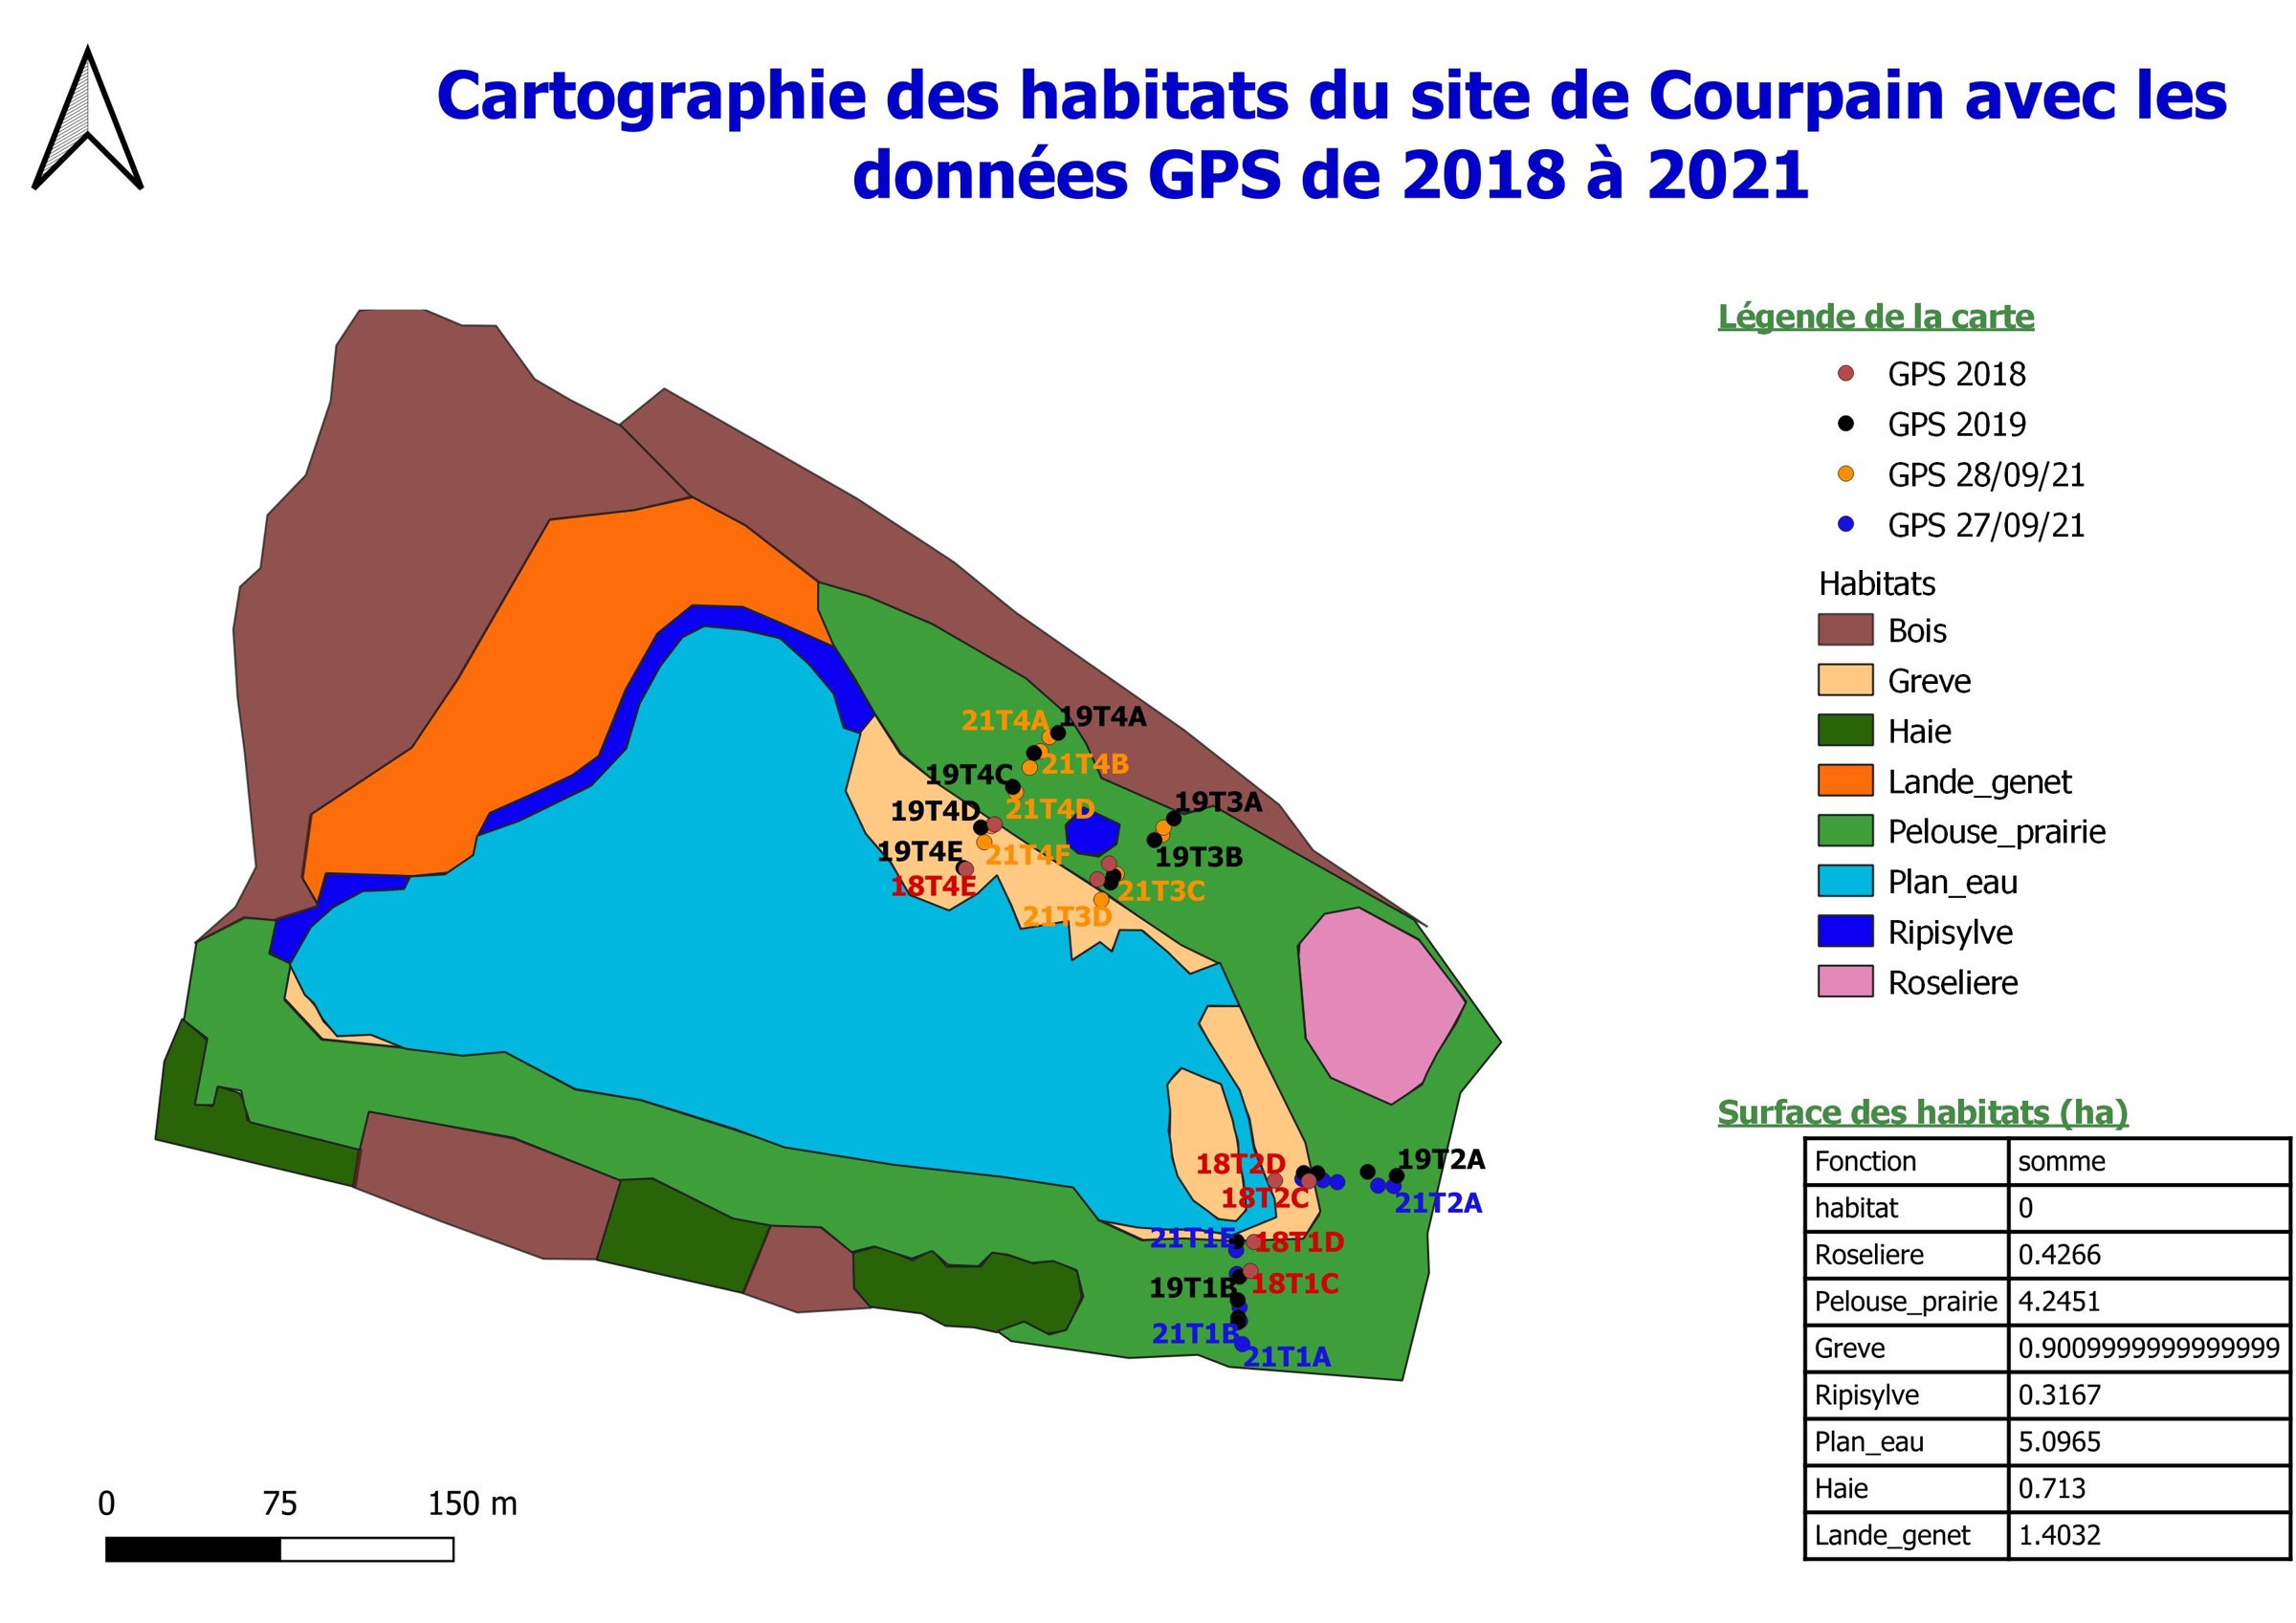
\includegraphics[width=\linewidth]{figures/carte_habitats.jpg}
\caption{Cartographie des habitats du site de Courpain et localisation des relevés GPS de 2018 à 2021 (QGIS).}
\label{fig:carte}
\end{figure}

\begin{table}[ht]
\centering\small
\caption{Surface des habitats cartographiés (ha). Les bois n'ont pas été mesurés.}
\label{tab:surfaces}
\begin{tabular}{@{}lr@{}}
\toprule\entete
Habitat & Surface (ha)\\
\midrule
Plan d'eau & 5,10\\
Pelouse et prairie & 4,25\\
Lande à genêts & 1,40\\
Grève & 0,90\\
Haie & 0,71\\
Roselière & 0,43\\
Ripisylve & 0,32\\
\bottomrule
\end{tabular}
\end{table}

\section{Méthodes d'analyse de la végétation}
\subsection{Relevés phytosociologiques}
Chaque relevé suit la méthode sigmatiste : liste des espèces et coefficient d'abondance-dominance \parencite{braunblanquet1932}. La surface du relevé est fixée par l'aire minimale \parencite{gounot1969} : on inventorie des quadrats emboîtés de surface croissante en notant les seules espèces nouvelles, jusqu'à ce que la courbe aire-espèces plafonne (figure~\ref{fig:releve}). Sur notre pelouse, l'aire minimale est de 8~m², pour 15 espèces. Les 45 relevés de 2018 à 2021 sont compilés dans un tableau brut de 124 taxons, avec leur type biologique \parencite{raunkiaer1934} et leur code phytosociologique Catminat \parencite{julve2017}.

\begin{figure}[ht]
\centering
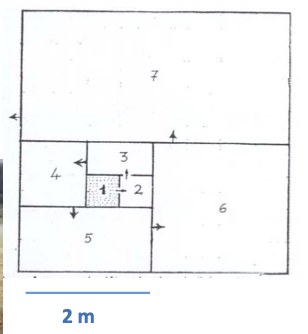
\includegraphics[height=48mm]{figures/schema_quadrats.jpg}\hspace{4mm}%
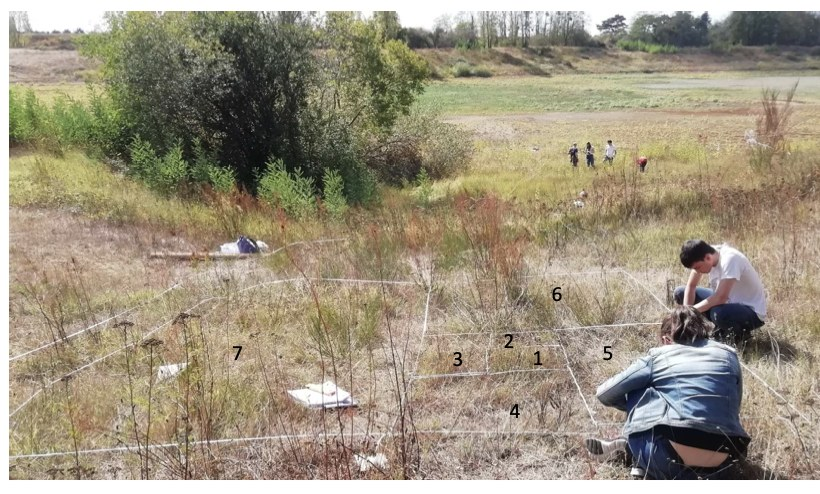
\includegraphics[height=48mm]{figures/photo_releve.jpg}
\caption{Méthode des quadrats emboîtés : ordre d'inventaire des surfaces croissantes (à gauche) et relevé sur le terrain (à droite).}
\label{fig:releve}
\end{figure}

\subsection{Analyses multivariées}
L'AFC \parencite{benzecri1973} projette relevés et espèces dans un même plan : deux relevés sont proches s'ils partagent les mêmes espèces, et une espèce se place près des relevés où on la trouve. Les axes sont ordonnés par la part de l'information (inertie) qu'ils expliquent. Un relevé fait d'espèces spécialistes d'un milieu s'écarte du centre ; un relevé d'espèces ubiquistes reste près du centre.

La CAH regroupe pas à pas les relevés les plus semblables et produit un dendrogramme ; le couper à un niveau de dissimilarité donne des groupes de relevés. Les deux analyses ont été refaites sous R (package \emph{vegan}) sur la présence-absence des espèces : AFC, puis CAH sur la distance de Jaccard avec le lien moyen.

\subsection{Fréquences et spectres biologiques}
Dans chaque groupe de relevés, la fréquence relative d'une espèce est $f_i = m_i / N$, avec $m_i$ le nombre de relevés où elle apparaît et $N$ le nombre de relevés du groupe. Les espèces sont rangées en classes de présence : I ($f_i \le 0{,}2$), II (0,2 à 0,4), III (0,4 à 0,6), IV (0,6 à 0,8) et V ($f_i > 0{,}8$) \parencite{gounot1969}. Les spectres biologiques comparent les types biologiques de deux façons : en présence (DQ, somme des fréquences de chaque type, en~\%) et en recouvrement (DRi, somme des recouvrements moyens, chaque coefficient étant remplacé par le centre de sa classe : 0,1~\% pour +, 2,5~\% pour 1, 15~\% pour 2, 37,5~\% pour 3, 62,5~\% pour 4, 87,5~\% pour 5).

\needspace{12\baselineskip}
\section{Résultats}
\subsection{AFC : un gradient d'humidité}
Les deux premiers axes expliquent 9,2~\% et 5,8~\% de l'inertie, soit 15,1~\% au total (figure~\ref{fig:afc}), une part modeste mais habituelle pour des données floristiques. L'axe~1 traduit le gradient d'humidité : les relevés humides sont à gauche, les relevés secs, très groupés, à droite. L'axe~2 isole la mégaphorbiaie, en haut. Le relevé 19T3b se détache seul : il porte des espèces qu'on ne trouve dans aucun autre relevé et forme un cas à part.

\begin{figure}[ht]
\centering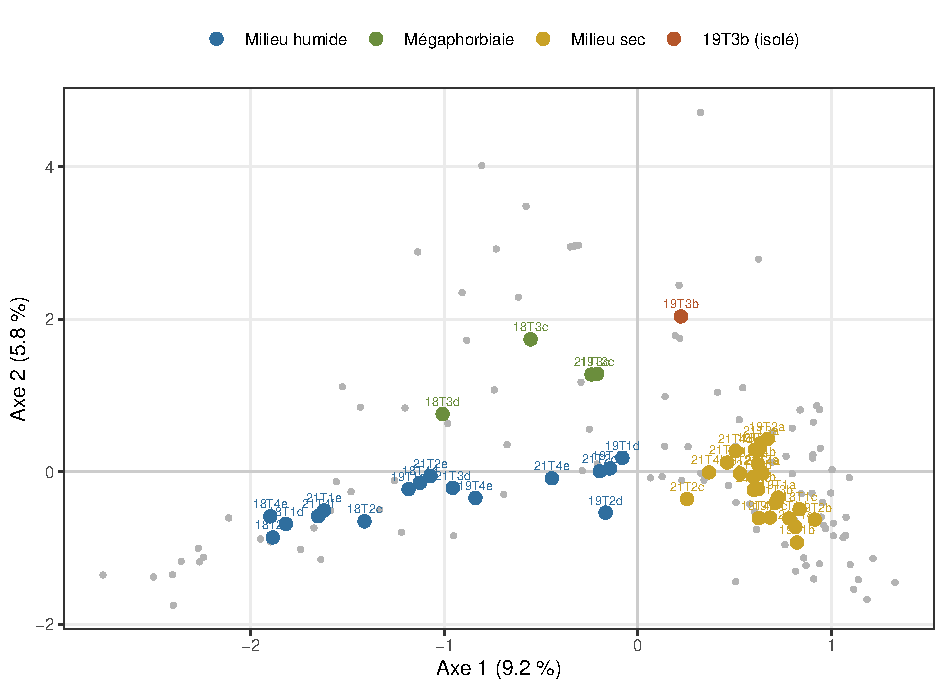
\includegraphics[width=0.92\linewidth]{figures/fig_afc.pdf}
\caption{AFC des 45 relevés (présence-absence) : relevés colorés selon leur groupe, espèces en gris.}
\label{fig:afc}
\end{figure}

\subsection{CAH : trois groupes de relevés}
Le dendrogramme sépare d'abord les relevés secs de tous les autres (figure~\ref{fig:cah}). Parmi ces derniers, la mégaphorbiaie se distingue des grèves humides. Les trois groupes retenus en 2021 sont donc retrouvés : milieu humide (16 relevés), mégaphorbiaie (4 relevés) et milieu sec (24 relevés), le relevé 19T3b restant à part.

\begin{figure}[ht]
\centering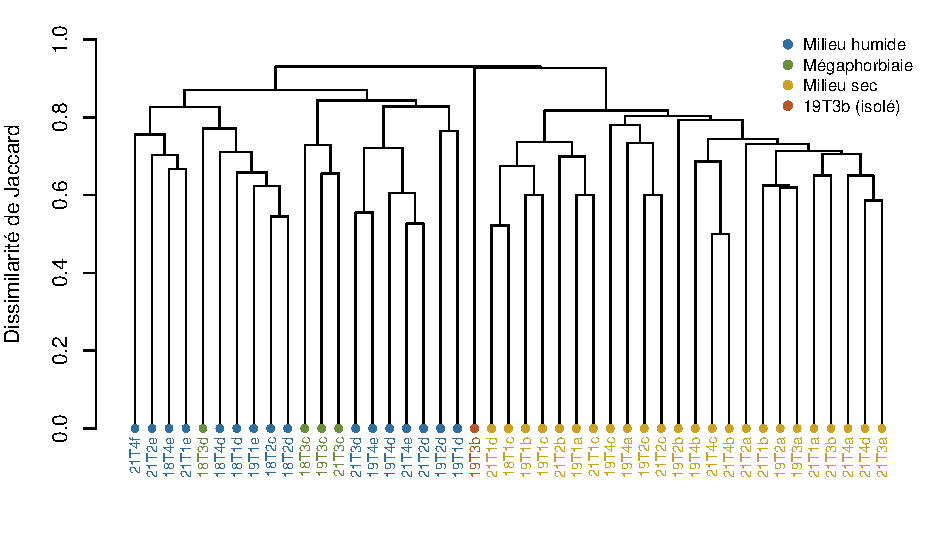
\includegraphics[width=\linewidth]{figures/fig_cah.pdf}
\caption{CAH des relevés (distance de Jaccard, lien moyen), feuilles colorées selon le groupe.}
\label{fig:cah}
\end{figure}

\subsection{Espèces et classes caractéristiques}
Les espèces les plus fidèles à chaque groupe, et leur classe phytosociologique Catminat, précisent l'écologie des trois milieux :
\begin{itemize}
\item \textbf{milieu humide} : \emph{Corrigiola littoralis}, \emph{Gnaphalium uliginosum}, \emph{Persicaria lapathifolia}, \emph{Rorippa sylvestris}, avec \emph{Xanthium strumarium} et \emph{Amaranthus blitum}. Ce sont des végétations annuelles des grèves exondées (\emph{Bidentetea tripartitae}, \emph{Juncetea bufonii}) mêlées de prairies inondables (\emph{Agrostietea stoloniferae}) ;
\item \textbf{mégaphorbiaie} : \emph{Phalaris arundinacea}, \emph{Lysimachia vulgaris}, \emph{Lycopus europaeus} (\emph{Phragmito-Magnocaricetea}), avec de jeunes \emph{Populus nigra} et \emph{Salix alba} qui annoncent la saulaie-peupleraie riveraine ;
\item \textbf{milieu sec} : \emph{Hypericum perforatum}, \emph{Oenothera biennis} (friches vivaces des \emph{Onopordetea}), \emph{Rumex acetosella} et \emph{Filago germanica} (pelouses pionnières sur sable, \emph{Koelerio-Corynephoretea}), \emph{Achillea millefolium} et \emph{Plantago lanceolata} (prairies), et \emph{Cytisus scoparius}, qui amorce la lande à genêts.
\end{itemize}

\noterevision{Note de révision (2026) : la version de 2021 attribuait les peupliers et saules à une « \emph{Stellarietea mediae} » (classe des cultures annuelles) et rangeait une classe de bas-marais parmi les pelouses sèches ; elle décrivait aussi le milieu sec comme basophile (pH > 7), en contradiction avec le pH de 5 mesuré. Ces points sont corrigés ici à partir des espèces caractéristiques de chaque groupe.}

\subsection{Histogrammes de fréquence}
Les histogrammes de présence ont une forme en L pour le milieu humide et le milieu sec (figure~\ref{fig:hist}) : la plupart des espèces sont en classe~I, présentes dans moins d'un relevé sur cinq. Ces deux groupes sont donc floristiquement hétérogènes, avec peu d'espèces communes à tous les relevés. La mégaphorbiaie, où les classes II et III dominent et où la classe~I est absente, est plus homogène ; elle ne compte cependant que quatre relevés, ce qui limite la portée du résultat.

\begin{figure}[ht]
\centering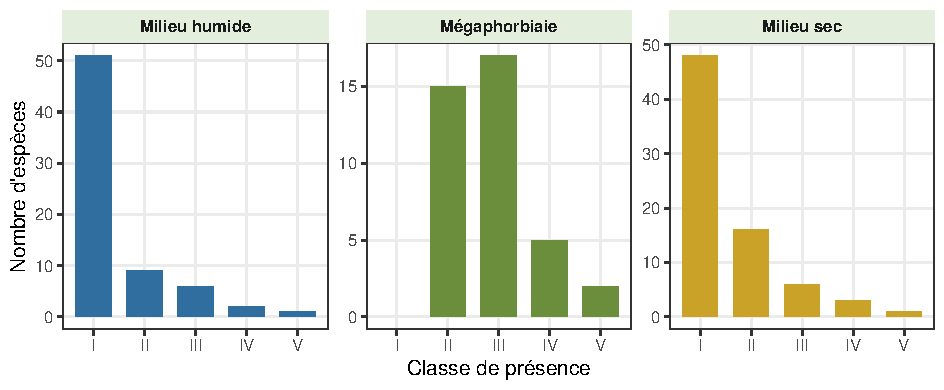
\includegraphics[width=0.85\linewidth]{figures/fig_histogrammes.pdf}
\caption{Histogrammes des classes de présence par groupe de relevés.}
\label{fig:hist}
\end{figure}

\noterevision{Note de révision (2026) : la version de 2021 lisait la classe~I comme des espèces annuelles. Elle regroupe en fait les espèces peu fréquentes, quel que soit leur type biologique ; l'interprétation est corrigée.}

\subsection{Spectres biologiques}
Le milieu humide est dominé par les thérophytes, plantes annuelles qui passent la mauvaise saison sous forme de graines : 62~\% en présence comme en recouvrement (figure~\ref{fig:spectres}). C'est la signature des grèves, découvertes chaque année par la baisse du niveau de l'eau puis recolonisées. La mégaphorbiaie et le milieu sec sont dominés par les hémicryptophytes, vivaces dont les bourgeons passent l'hiver au ras du sol (51 et 71~\% en présence). Dans le milieu sec, elles couvrent même 82~\% de la surface. La mégaphorbiaie compte aussi des géophytes et des phanérophytes, les jeunes arbres de la future ripisylve.

\begin{figure}[ht]
\centering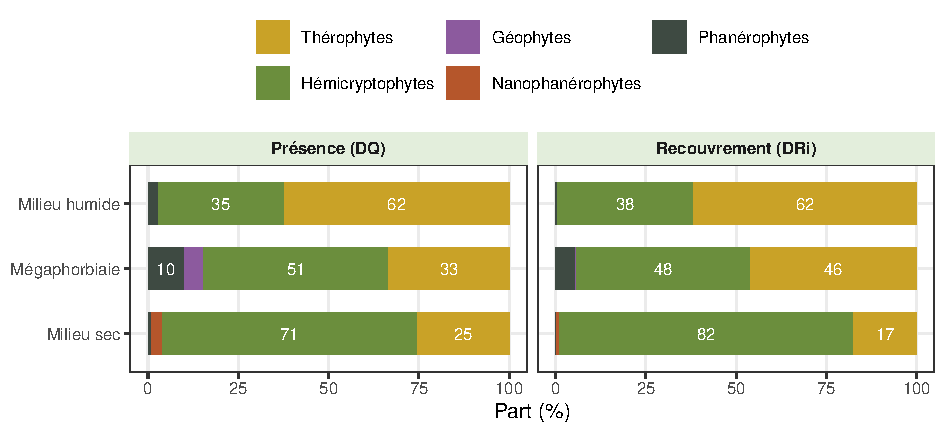
\includegraphics[width=0.9\linewidth]{figures/fig_spectres.pdf}
\caption{Spectres biologiques par groupe : présence (DQ) et recouvrement (DRi), en pourcentage.}
\label{fig:spectres}
\end{figure}

\section{Conclusion}
Les analyses concordent : la végétation de Courpain s'organise selon le gradient d'humidité qui part du plan d'eau. Trois ensembles se dégagent. Les grèves humides, pionnières et dominées par les annuelles, sont remaniées chaque année par les variations du niveau de l'eau. La mégaphorbiaie à hautes herbes évolue vers la saulaie-peupleraie. Les pelouses sèches, sur sable acide, sont dominées par les vivaces et colonisées par le genêt.

Sans intervention, la mégaphorbiaie et les pelouses évolueraient vers des fourrés puis des boisements. La fauche annuelle pratiquée par le gestionnaire maintient les milieux ouverts et la mosaïque d'habitats qui fait l'intérêt du site pour les oiseaux. Plus de relevés en mégaphorbiaie et un suivi régulier des mêmes points permettraient de suivre cette dynamique.

\pagebiblio
\end{document}
